\documentclass[SDSUThesis.tex]{subfiles} 
\begin{document}

% All about the SDLC Analytic Engine
\section{SDLC ANALYTIC ENGINE}
\label{sec:SDLC-AE}

In order for an SDO to properly track the elements of CRI, a data storage system should be available to store the appropriate data.  A consistent storage system should help to avoid the problem of inaccurate
data caused by numerous manipulations of the existing data \cite{Olson2003}. Plus, if the system
is implemented correctly by allowing limited changes to existing data, it will be able to alleviate
some of the dishonesty that is currently present in software projects \cite{Rost2011}. This storage system will be named the SDLC Analytic Engine (SDLC-AE). Figure \ref{fig:sdlc-ae} provides an overview of the data that could potentially be stored in the SDLC-AE.


Once all the SDLC data is collected into a single place, there are many possible applications.  Software analytics
will be much easier to create and gamification will be much more easily attainable.  

\begin{figure}[ht]
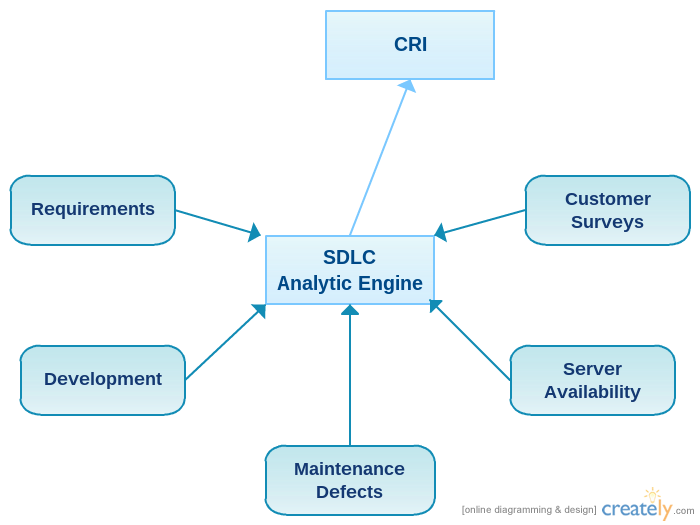
\includegraphics[scale=.6]{images/sdlcae.png}
\caption{SDLC ANALYTIC ENGINE}
\label{fig:sdlc-ae}
\end{figure}

\subsection{DATABASE STRUCTURE}
   All the data necessary to compute CRI needs to be stored in a database.  This section will 
   lay out the structure of tables and relationships necessary to the store all the data
   within a relational database.  
   
   \subsubsection{TABLES FOR RAW CRI DATA}
   
        The first set of tables that need to be created are tables
        to store the raw data that is collected.  These tables
        will line up with the necessary data for each of the 5 elements
        of CRI.  Figure \ref{fig:raw} provides a visual description
        of the tables that are needed.  The tables have no relationship
        with each other since they are raw data.  The primary goal of
        these tables is to store the raw data in a single database. The
        5 table names are:
        \begin{enumerate}
            \item QUALITY\_RAW
            \item AVAILABILITY\_RAW
            \item SATISFACTION\_RAW
            \item SCHEDULE\_RAW
            \item REQUIREMENTS\_RAW
        \end{enumerate}
        Notice these table names match with the 5 elements of CRI.
   
       \begin{figure}[ht]
            \centering
            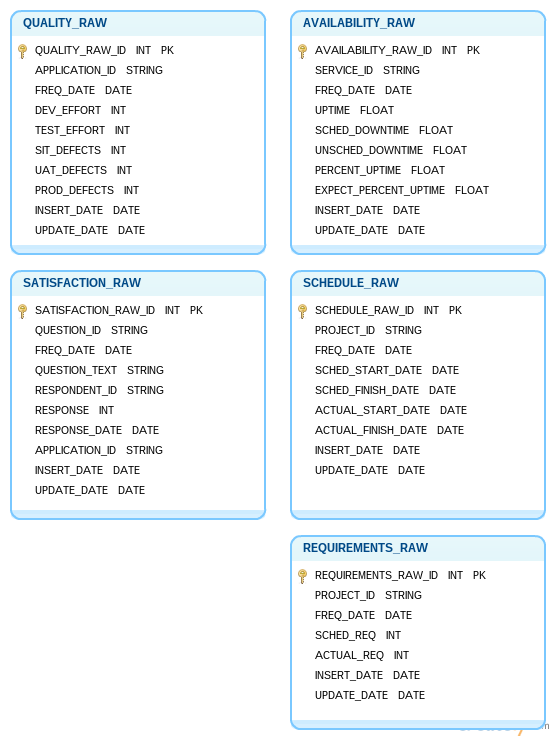
\includegraphics[scale=.55]{images/raw_tables.png}
            \caption{TABLES FOR RAW CRI DATA}
            \label{fig:raw}
        \end{figure}
        
        Appendix \ref{src:rawSQL} provides the necessary SQL statements to create the 
        database tables for storing the raw CRI data.  The SQL is written for an Oracle
        database, but the scripts can be modified to work with another database
        such as: PostgreSQL, SQL Server, or MySQL.  
        
    \subsubsection{INTERMEDIATE SCORE TABLES FOR CRI}
    
        Appendix \ref{src:scoreSQL} provides the necessary SQL statements to create the 
        database tables for storing the intermediate CRI scores.
        
       \begin{figure}[ht]
            \centering
            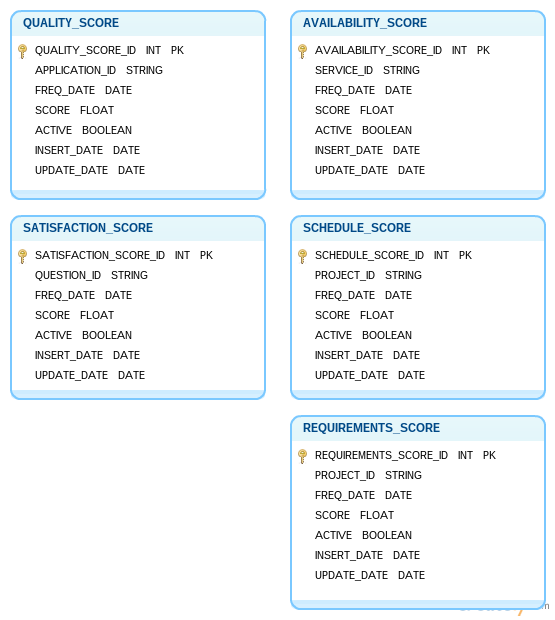
\includegraphics[scale=.55]{images/score_tables.png}
            \caption{TABLES FOR INTERMEDIATE CRI SCORES}
            \label{fig:score_tables}
        \end{figure}%
    
    \subsubsection{FINAL SCORE TABLES FOR CRI}
    
        Appendix \ref{src:overallscoreSQL} provides the necessary SQL statements to create the 
        database tables for storing the final scores for each element and the final 
        overall CRI scores for each time frequency.
        
       \begin{figure}[ht]
            \centering
            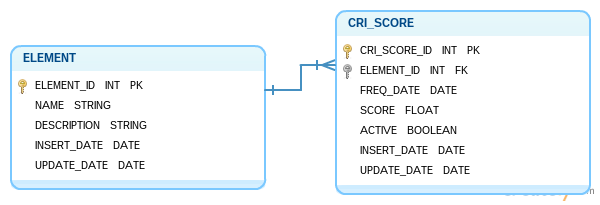
\includegraphics[scale=.55]{images/final_score_tables.png}
            \caption{TABLES FOR FINAL CRI SCORES}
            \label{fig:final_score_tables}
        \end{figure}

\subsection{QUERIES}
    The section will provide the necessary SQL queries to obtain the correct data
    needed to compute the individual elements of CRI.
    
\subsection{COMPUTATIONS}
    This section will provide R scripts to calculate each individual score and the overall 
    CRI score. The scripts will need to be run every time the data is updated and the CRI
    score needs to be recalculated.
    
    

making decisions based upon historical data. 
Data Driven Software Engineering not Data Driven Software Development


\end{document}







